\documentclass[10pt, twocolumn]{article}
\usepackage[margin=1in]{geometry}
\usepackage{graphicx}
\usepackage{microtype}
\usepackage{verbatim}
\usepackage{amsmath}
\usepackage{nicefrac}
\usepackage[colorlinks=false, hidelinks]{hyperref}
\usepackage{caption}
\usepackage{subcaption}
\usepackage{listings}

\title{%
	\makebox[\textwidth][s]{%
		\hfill
		\begin{tabular}[b]{@{}c@{}}
				\fontsize{14}{20}\bfseries\selectfont \emph{Easy--PCB} Solder Reflow Oven\\
				\fontsize{12}{18}\selectfont Ben Lorenzetti\\
 		\end{tabular}%
    		\hfill
    		\makebox[0pt][r]{%
      			\includegraphics[width=0.2\textwidth]{Figures/easy-pcb-oven.pdf}}%
 	}% end makebox
}% end title

\author{}
\date{}

\begin{document}

\maketitle

\section*{Features}
\addcontentsline{toc}{section}{Features}

\begin{flushleft}
	\begin{itemize}
		\fontsize{10}{12}\bfseries\selectfont
		\item Insulated aluminum frame with XxYxZ interior chamber
		\item XXX Watt heating element with solid state relay control
		\item Forced convection fan driven by bipolar stepper motor with speed control
		\item Type X thermocouple for temperature feedback loop
		\item XXXXX based feedback control
		\item Integrated 120 VAC power supply with surge and short protection
		\item Combined temperature/run time \mbox{7--segment} display
		\item Convenient pushbutton/menu interface for temperature profile programming
	\end{itemize}
\end{flushleft}

\section*{Introduction}
\addcontentsline{toc}{section}{Introduction}

\emph{Easy--PCB} is a small, desktop convection oven for DIY reflow soldering at home.

As integrated circuits continue to become smaller and faster,
many $\mu$--controllers, FPGAs, and other ICs are no longer available in
DIP form for breadboard prototyping or solder iron soldering.
Similar to the shift away from PC parallel ports in the early 2000s,
the shift away from DIPs means modern electronics hobbyists need more
complicated equipment than their predessesors.

Currently, commercial solder reflow stations are available for
soldering fine pitch, SMD, and BGA componenets.
More recently, several hackers have created open source designs
for inexpensive reflow ovens, using converted kitchen toaster ovens.

\emph{Easy--PCB} is better because it is a convection oven;
controlled air flow prevents parts from being blown out of position and
convection heating obviates the uneven heat absorbtion seen in infrared radiation based systems.
Furthermore, \emph{Easy--PCB} was designed from the ground up for soldering,
so the heating elements and oven frame were optimized alongside the
temperature controller for a typical solder reflow profile.

\begin{center}
	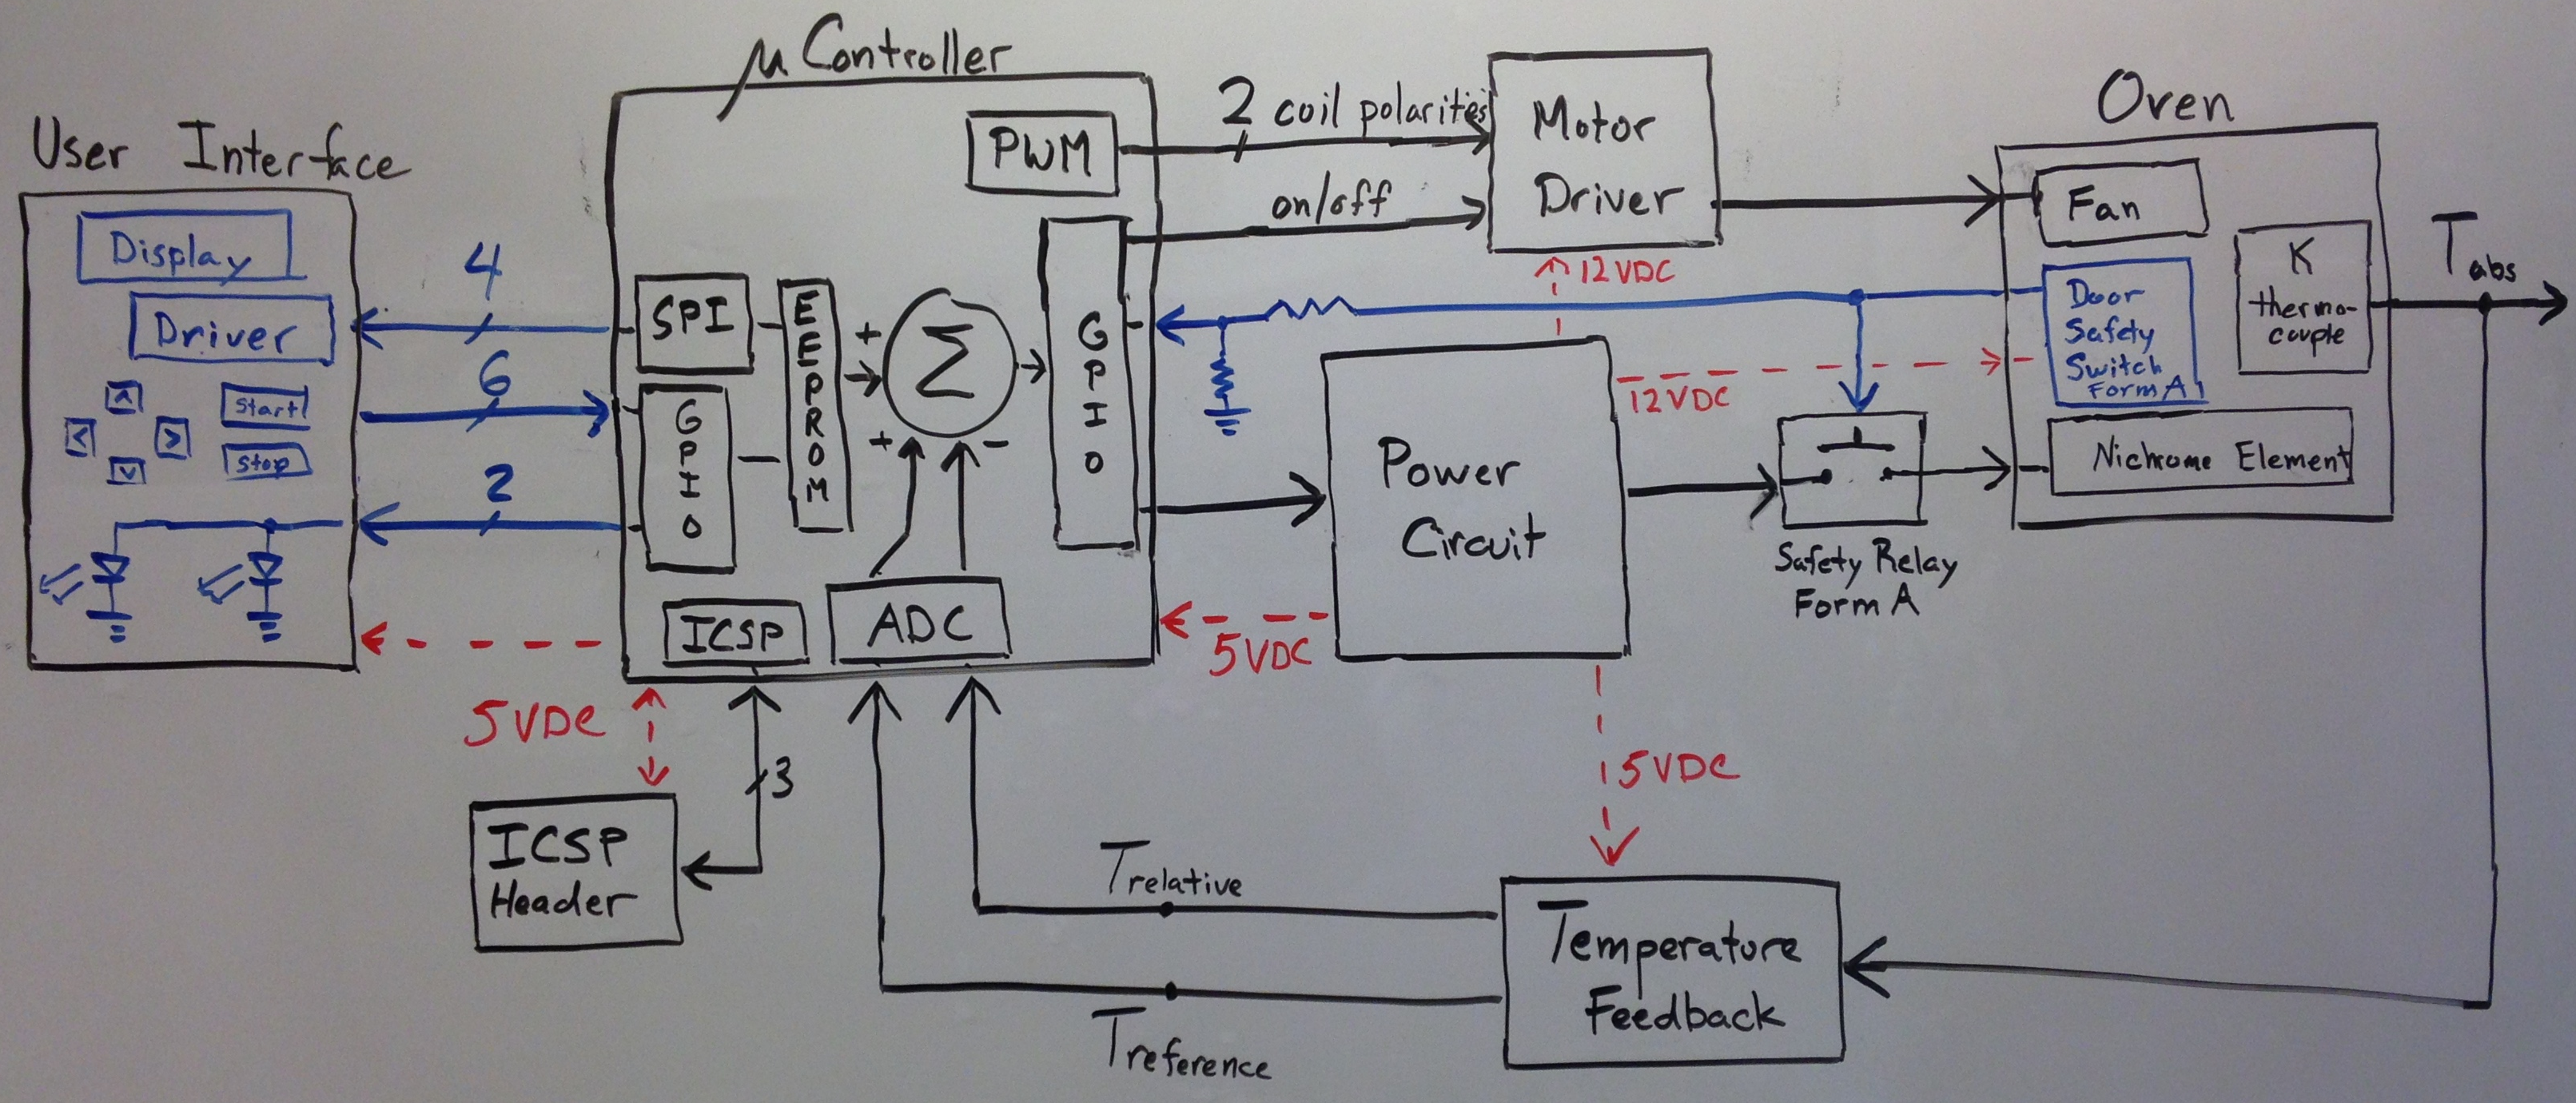
\includegraphics[width=\columnwidth]{Figures/control-system.pdf}
	\captionof*{figure}{The \emph{Easy--PCB} Control System: not just a controller bolted onto a disjoint oven.}
\end{center}

\emph{Easy--PCB} allows hobbyists to produce solder reflow temperature profiles with
a high degree of accuracy and repeatability.
Alongside freely available PCB design programs like Eagle and low-quantity
fabrication services like OSH Park, \emph{Easy--PCB} makes
modern integrated components, such as digital CMOS cameras,
within the range of capabilities of independent hobbyists.

\begin{center}
	\includegraphics[width=\columnwidth]{Figures/control-results.pdf}
	\captionof*{figure}{Faithful Temperature Profile Control}
\end{center}

\tableofcontents

\section{User Interface}

\section{Plant Design}

\subsection{Temperature Objectives}

\subsection{Thermodynamics Theory}

The heat required to increase temperature of a unit mass of material by one degree is
\begin{equation}
dQ=mc_{p}dT
\label{specific-heat-eq}
\end{equation}
where \(c_{p}\) is the specific heat of the material with \mbox{units \(\left[\frac{kJ}{kg*K}\right]\)}.

\begin{equation}
\vec{q}=-k\vec{\nabla}T
\label{fouriers-law-differential-form}
\end{equation}
where \(k\) is thermal conductivity with \mbox{units \(\left[\frac{W}{m*K}\right]\)}.

\begin{equation*}
\frac{dQ}{dt}=-k\oint _{S}\vec{\nabla}T*d\vec{A}
\end{equation*}
where \(d\vec{A}\) is a differential area element of a closed \mbox{surface \(S\)}.

\begin{equation}
\frac{\delta Q}{\delta t}=-kA\frac{\delta T}{\delta x}
\label{fouriers-law-in-1D}
\end{equation}

\begin{equation}
\frac{dQ}{dt}=hA\Delta T
\label{newtons-cooling-law}
\end{equation}
where \(h\) is the heat transfer coefficient with \mbox{units \(\left[\frac{W}{m^{2}*K}\right]\)}.

\subsection{Conceptual Design}

Most microwaves draw between 600 and 1200 Watts of power.
An IR toaster oven may draw 1500 Watts into its lamps.
How much power does \emph{Easy-PCB} need to produce the required temperature profiles?

Our approach for answering this question is to browse available parts on McMaster.com,
imagine how they would be assembled into an oven,
and then model their thermodynamic responses using PSPICE.
Thermodynamics can be modeled in SPICE because temperature is
mathematically analogous to voltage (both are potential functions)
and heat energy to electric charge.

Starting from the source of heat and moving towards the heat sinks,
the first component in a convection oven is a heating element.
Most electric heating elements are protected from shorts and moisture
by a metal sheath.
If the sheath is relatively thin compared to the square root of its surface area,
then its heat transfer can be modeled as a 1--D transmission line, like shown in
\hyperref[sheath-transmission-line]{figure \ref{sheath-transmission-line}}.

\begin{figure}
\centering
\includegraphics[width=0.9\columnwidth]{Figures/sheath-transmission-line.pdf}
\caption{One--Dimensional Model of Heating Element Sheath}
\label{sheath-transmission-line}
\end{figure}

From \hyperref[specific-heat-eq]{equation \ref{specific-heat-eq}},
the heat capacity of a thin slice of the metal sheath is
\begin{equation*}
dQ=(\rho A dx)c_{p}dT
\end{equation*}

And, using Fourier's Law of heat conduction in 1--D,
(\hyperref[fouriers-law-in-1D]{equation \ref{fouriers-law-in-1D}})
the rate of heat passing through a thin slice is
\begin{equation*}
\frac{\delta Q}{\delta t}=kA\frac{\delta T}{\delta x}
\end{equation*} 
 
Rewriting these equations to look like current-voltage relationships gives
\begin{equation}
\delta T=R_{x}\frac{\delta Q}{\delta t},
\quad R_{x}=\frac{\delta x}{kA}
\label{differential-resistance-eq}
\end{equation}
and
\begin{equation}
\frac{\delta Q}{\delta t}=C_{x}\frac{\delta T}{\delta t},
\quad C_{x}=\rho A c_{p} * \delta x
\label{differential-capacitance-eq}
\end{equation}

Values for $k$, $c_{p}$, and $\rho$ of different metals are listed in
\hyperref[thermal-properties-table]{table \ref{thermal-properties-table}}.

Long metal bars and rods can also be modeled with equations
\ref{differential-resistance-eq} and \ref{differential-capacitance-eq}
if the heat loss along the length of the bar is assumed to be
negligible compared to heat transfered at the end faces.

For sheaths or metal bars where heat is injected at the center
of the part and dissipates symmetrically in either direction,
the surface area can be doubled so that the transmission line
only needs to be integraded in the positive direction.
\begin{equation}
\left\{\begin{array}{c c c}
R_{x}	&\Rightarrow	&R_{x}/{2}	\\
C_{x}	&\Rightarrow	&2C_{x}	\\
\{x|-\frac{w}{2} \leq x \leq \frac{w}{2}\}	&\Rightarrow	&\{x|0 \leq x \leq \frac{w}{2}\}	\\
\end{array}\right.
\end{equation}

\begin{table*}
\centering
\caption{Thermal Conductivity, Specific Heat, and Density of Selected Materials}
\begin{tabular}{c | c | c | c | c}
\hline\hline
Material	&Linear Region (K--K)	&k \(\left(\frac{W}{m*K}\right)\)	&\(c_{p}\) \(\left(\frac{kJ}{kg*K}\right)\)	&\(\rho\) \((kg/m^{3})\)	\\
% Material	Linear Region		k	Cp	density	\\
\hline\hline

\hline\hline
\end{tabular}
\label{thermal-properties-table}
\end{table*}

At any moment in time, we can plot the temperature of air as one
moves away from the sheath surface. We see there is a certain
distance, called the skin depth $\delta$, over which the temperature
gradient is nearly dissipaited and the bulk air begins.

PLOT with T0et/alpha and Tbulk on y axis and x on x axis

Forced convection from the fan causes the bulk air, uniform temperature
region to be pushed closer to the sheath's surface.
If the skin depth can be pushed sufficiently close to the surface,
then the time constant shrinks due to the relation $\alpha=\frac{k}{\rho c_{p}}\delta$.
Thus, for sufficiently strong circullation and close skin depth, the time
constant becomes small enough that the system is effectively always in
steady state, where
\begin{equation*}
\frac{dT}{dt}\approx 0
\end{equation*}

From the first law of thermodynamics (conservation of energy),
the difference between heat flowing in and out of a thin slice by
all mechanisms is equal to the heat stored within that slice, for all t and x.
\begin{equation*}
\frac{\delta Q_{\textrm{cap.}}}{\delta t}*\frac{1}{\delta x}=
\frac{\delta Q_{\textrm{cond.}}}{\delta t}*\frac{1}{\delta x}+
\frac{\delta Q_{\textrm{conv.}}}{\delta t}*\frac{1}{\delta x}
\end{equation*}

Substituting
\hyperref[differential-capacitance-eq]{equation \ref{differential-capacitance-eq}}
for the heat capacity of a thin slice yields:

\begin{equation*}
\rho A c_{p}\frac{\delta T}{\delta t}=
\frac{\delta Q_{\textrm{cond.}}}{\delta t}*\frac{1}{\delta x}+
\frac{\delta Q_{\textrm{conv.}}}{\delta t}*\frac{1}{\delta x}
\end{equation*}

But we have just argued that if the skin depth can be made very close
by forced convection, then $\frac{dT}{dt}\rightarrow 0$.

\begin{equation*}
\frac{\delta Q_{\textrm{conv.}}}{\delta t}*\frac{1}{\delta x}=-
\frac{\delta Q_{\textrm{cond.}}}{\delta t}*\frac{1}{\delta x}
\end{equation*}

Integrating across x is easy.

\begin{equation*}
\frac{dQ_{\textrm{conv.}}}{dt}(x)=C-
\frac{dQ_{\textrm{cond.}}}{dt}(x)
\end{equation*}

At the surface of the sheath \((X=0)\), heat transfer in the air is
100\% conduction because every air molecule at \((X=0)\) is colliding
with metal and exchanging energy. Therefore
\begin{equation*}
C=\frac{dQ_{\textrm{cond.}}}{dt}(X=0)
\end{equation*}

Applying Fourier's Law to the temperature profile found in
\hyperref[conduction-temp-profile]{equation \ref{conduction-temp-profile}}
give us equations for the rate of heat tranfer due to conduction,
and finally this leads to
\begin{equation*}
\dot{Q}_{\textrm{cond.}}(x)=Q_{0}e^{\nicefrac{-x}{\delta}}
\end{equation*}
and
\begin{equation*}
\dot{Q}_{\textrm{conv.}}(x)=Q_{0}\left(1-e^{\nicefrac{-x}{\delta}}\right)
\end{equation*}

where
\begin{equation*}
Q_{0}=\frac{kAT_{0}}{\delta}e^{\nicefrac{-t}{\alpha}}
\end{equation*}

Finally, if we absorb $e^{\nicefrac{-t}{\alpha}}$ into $T_{0}$ for steady state, then
\begin{equation}
Q_{0}=\frac{kA}{\delta}T_{0}
\end{equation}





\subsection{Component Selection \& SPICE Modeling}

\subsection{Transfer Model}

\section{Thermocouple Amplifier Design}

\subsection{Controller and Power Requirements}

\section{Motor Driver Design}

\subsection{Power Requirements}

\section{Power Circuit Design}

\section{Controller Design}

\end{document}
